\documentclass[11pt]{article}
\usepackage[T1]{fontenc}
\usepackage[utf8]{inputenc}
\usepackage{lmodern}
\input{glyphtounicode}
\pdfgentounicode=1
\usepackage{amsmath,amssymb,amsthm,geometry,hyperref,multicol,fancyvrb}
\usepackage{graphicx}
\usepackage{tikz}
\usepackage{float}
\usepackage{needspace}
\usepackage[title]{appendix}
\geometry{margin=1in}
\setlength{\emergencystretch}{3em}
\hypersetup{colorlinks=true,linkcolor=blue,citecolor=blue,urlcolor=blue,pdftitle={A planar graph without four- or nine-cycles that is not three-colorable},pdfauthor={P. Graham},pdfsubject={Computer-assisted graph coloring counterexample},pdfkeywords={planar graph, proper coloring, forbidden cycles}}
\newtheorem{theorem}{Theorem}
\newtheorem{lemma}{Lemma}
\newcommand{\file}[1]{\texttt{\detokenize{#1}}}
\title{A planar graph without four- or nine-cycles\texorpdfstring{\\}{ }that is not three-colorable}
\author{P. Graham\\ \small\url{https://orcid.org/0009-0007-8493-1505}}
\date{October 25, 2026}
\begin{document}
\maketitle
\begin{abstract}
Lu, Wang, Wang, Bu, Montassier and Raspaud asked which cycle lengths, together with length four, force
proper three-colorability of planar graphs, as recorded by Kang, Jin and
Wang. Cohen-Addad, Hebdige, Král',
Li and Salgado disproved Steinberg's conjecture for lengths four and five.
Kostochka and Yancey proved a sharp general lower bound on the number
of edges of a four-critical graph. We give an 82-vertex planar graph
without cycles of length four or nine that is four-critical and attains
that bound, answering the length-nine case of that question.
The graph is obtained by Dirac--Haj\'os--Gallai--Ore compositions of complete four-vertex graphs.
Its non-three-colorability follows by induction on this construction;
a rotation system, cycle enumeration and three-colorings after edge deletion establish
the remaining properties. Lean verifies the rotation certificate, the
exclusion of four- and nine-cycles, and non-three-colorability of the
same graph.
\end{abstract}

\section{Introduction}
All graphs in this paper are finite and simple. A proper three-coloring
is a map $f:V(G)\to\{0,1,2\}$ with $f(u)\ne f(v)$ for every edge $uv$.
A cycle is simple; it need not be induced. Thus forbidding a cycle of
length $k$, denoted $C_k$, forbids cycles with chords as well.

A graph is \emph{four-critical} if it has chromatic number four and
every proper subgraph is three-colorable.
Ore composition is the edge deletion and vertex splitting operation defined
in Section~\ref{sec:ore}. A graph obtained from copies of $K_4$ by Ore
compositions is called a \emph{four-Ore graph}~\cite[Section 1]{ky}.
A rotation system specifies the cyclic order of the neighbors at each vertex.
For a graph $G$, write $\chi(G)$ for its chromatic number and $G-e$ for
the graph obtained by deleting edge $e$.

Steinberg conjectured in 1976 that every planar graph without $C_4$ or
$C_5$ is properly three-colorable; see the account in~\cite[opening paragraph]{steinberg}.

\begin{theorem}\label{thm:main}
There exists an 82-vertex planar graph with 136 edges, without cycles of
length four or nine, that is four-critical and is not properly three-colorable.
It is a four-Ore graph and has the fewest edges among all 82-vertex
four-critical graphs.
\end{theorem}

The theorem gives a negative answer to the $i=9$ case of Kang, Jin and Wang's
Problem 1.2~\cite{kjw}, which asks which $i\in\{5,6,7,8,9\}$
make every planar graph without $C_4$ or $C_i$ properly three-colorable.
Kang, Jin and Wang write that a more general problem ``was formulated
also in [7]''~\cite[Section 1, immediately before Problem 1.2]{kjw}; their
reference [7] is Lu, Wang, Wang, Bu, Montassier and Raspaud~\cite{lu}. Cohen-Addad, Hebdige, Král', Li and Salgado's
counterexample to Steinberg's conjecture concerns $C_4,C_5$~\cite[Theorem 3]{steinberg};
its Figure 1 contains the nine-cycle described below.
Our graph answers the $C_4,C_9$ question using Ore composition and attains
Kostochka and Yancey's edge bound~\cite[Theorem 3]{kybound}.
The contribution is the explicit graph for the length-nine case; the
Ore-composition argument and the critical-graph edge bound are the tools.
The difficult construction step was to choose identifications between small
planar pieces that make their possible proper three-colorings incompatible
without creating the forbidden cycles. The restrictions of a piece's
three-colorings to the vertices to be identified form a finite list of
color patterns. Composing these lists determines which identifications
are incompatible with three-colorability; the cycle restrictions must
also hold for the resulting graph. The identifications were found by a
computer search: small planar pieces were classified by these color patterns,
and their compositions were continued until no coloring pattern remained.
For the resulting
graph, Ore composition gives the short proof of non-three-colorability
below; the rotation and exhaustive cycle enumeration establish planarity
and the cycle exclusions. Section~\ref{sec:ore} illustrates
the first composition and gives the proof; the complete construction is
printed in Appendix~\ref{app:ore}.

\paragraph{Related coloring results.}\label{app:scope}
Nearby results on proper, list and defective coloring put the forbidden-pair question in context.

We observe that the $G_1$ component in Figure 1 of Cohen-Addad and
coauthors~\cite{steinberg} contains the nine-cycle
$a,f,k,n,m,j,i,h,g,a$ in the paper's own labels. This component is retained
in the published construction~\cite[Lemma 2 and proof of Theorem 3]{steinberg}.


Here DP-coloring means correspondence coloring~\cite[Section 1]{kjz}.

Kang, Jin and Wang prove proper three-colorability when $C_6$ is also
excluded~\cite[Theorem 1.4]{kjw}. The $\{C_4,C_7,C_9\}$-free class is properly three-colorable by Lu and
coauthors, as also recorded in~\cite[Section 1, paragraph following Problem 1.3]{kjw}; Kang, Jin and Zhu prove
DP-3-colorability of that class~\cite[Theorem 1.1]{kjz}.
Their Corollary 1.2 states that these graphs are
``3-choosable (and hence 3-colorable)''~\cite{kjz}.


Defective colorings are a different
notion: a $(d_1,d_2,d_3)$-coloring permits each color class to induce
maximum degree at most $d_j$.
Related work includes Jin, Kang, Liu and Wang on $(1,0,0)$-colorability~\cite[Theorem 1.4]{jklw}.
For the four-and-nine pair, Dai, Wang and Xu's title is
``Every planar graph without cycles of length 4 or 9 is $(1,1,0)$-colorable''~\cite{dai},
while Chen, Dai, Nie, Wang and Yu study $(2,0,0)$-colorability~\cite[Theorem 1.4]{nie}.
Xiao and Huang's article is entitled
``A weak DP-coloring of planar graphs without 4- and 9-cycles''~\cite{xiao}.
Jin, Kang, Liu and Wang described the cases $i\in\{6,7,8,9\}$ as
``still unsettled''~\cite[paragraph following Problem 1.2]{jklw}.
For further bibliographic context see Ang and Leo~\cite{ang}, Bu, Wang
and Wang~\cite{survey}, and Li, Niu and Tian~\cite{bordeaux}.

The proof depends on finite computations described in
Section~\ref{sec:checks}, together with the written arguments below.
The proofs, the Lean formalization, the search code, the certificate checkers
and the text were produced by AI models (from OpenAI and Anthropic), working
under the author's direction. This paper is computer-assisted and has not
yet been reviewed by experts.

\section{Construction and proof}\label{sec:ore}
The graph $G$ has vertex set $\{0,\ldots,81\}$. We prove
non-three-colorability by constructing $G$ from copies of $K_4$ by Ore
composition. A rotation system proves planarity, and enumeration excludes
the forbidden cycles. Proper three-colorings of $G-e$ for every edge $e$ establish four-criticality;
the number of edges then gives equality in the cited lower bound.



\Needspace{9\baselineskip}
For a graph $B$, $N_B(z)$ denotes the set of neighbors of vertex $z$.
We use the name Ore composition for the operation called
DHGO-composition in Kostochka and Yancey's Section 1~\cite{ky}.

\begin{samepage}
Take vertex-disjoint graphs $A$ and $B$, an edge $xy$ of $A$, and a
vertex $z$ of $B$. Partition $N_B(z)$ into two nonempty disjoint sets
$N_x,N_y$. Delete $xy$ from $A$, replace $z$ in $B$ by two nonadjacent
vertices, and identify those vertices with $x,y$, respectively, assigning
neighbors $N_x$ to $x$ and $N_y$ to $y$. The resulting graph is an
\emph{Ore composition}, also called a Dirac--Haj\'os--Gallai--Ore (DHGO)
composition~\cite[Section 1]{ky}.
\end{samepage}

The key point is that a three-coloring of an Ore composition of two
non-three-colorable graphs would force the ends of the deleted edge to
have the same color: different colors would give a three-coloring of the
first graph. Their common color could then be assigned to the split
vertex of the second graph, giving another contradiction. Lemma~\ref{lem:ore}
makes this argument precise, so induction from $K_4$ proves
non-three-colorability. The cycle restrictions are established separately
for the resulting graph by the two complete enumerations in
Appendix~\ref{app:cycles}.

Appendix~\ref{app:ore} represents the construction as a rooted tree of compositions.
Tree-node numbers index construction instructions; vertex labels name the
vertices in their operands. These are distinct columns of the construction
table. Labels at least 82 are temporary split vertices;
none survives at the root, node 52.
The first composition in the construction uses copies of $K_4$ on
$\{12,60,62,84\}$ and $\{13,61,63,85\}$. It deletes the edge $62\,84$,
splits vertex $85$, and assigns neighbor $63$ to $62$ and neighbors $13,61$
to $84$. Figure~\ref{fig:ore-step} shows this operation. This is the first internal
row of the tree in Appendix~\ref{app:ore}; its later rows specify every
subsequent identification. Write $J_t$ for the graph specified at node $t$ of that table. The last
composition deletes edge $0\,7$ from $J_{28}$ and splits vertex 82 of
$J_{51}$: neighbors $2,3,4,5$ are attached to 0 and neighbors $8,9,10,11$
to 7. Its two operands are obtained from $J_4,J_{27}$ and $J_{47},J_{50}$,
respectively, as shown in Figure~\ref{fig:ore-tree}. These are construction
indices, distinct from vertex labels. Figure~\ref{fig:graph} in
Appendix~\ref{app:rotation} shows the full graph.

\begin{figure}[H]
\centering
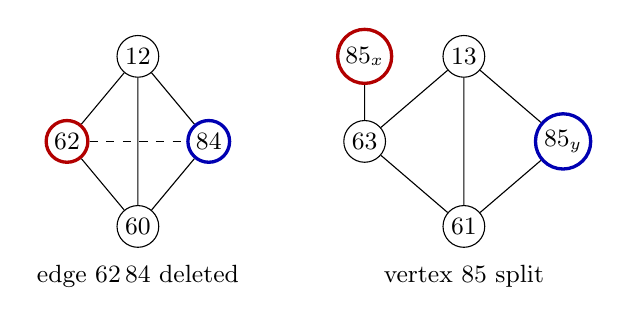
\begin{tikzpicture}[scale=.90,every node/.style={font=\small},
 orevertex/.style={circle,draw,fill=white,inner sep=1.5pt},
 orex/.style={orevertex,draw=red!70!black,very thick},
 orey/.style={orevertex,draw=blue!70!black,very thick}]
\node[orex] (ax) at (-2,0) {62};
\node[orey] (ay) at (0,0) {84};
\node[orevertex] (a12) at (-1,1.2) {12};
\node[orevertex] (a60) at (-1,-1.2) {60};
\draw[dashed] (ax)--(ay);
\draw (a12)--(a60) (a12)--(ax) (a60)--(ax)
      (a12)--(ay) (a60)--(ay);
\node at (-1,-1.9) {edge $62\,84$ deleted};
\node[orex] (bx) at (2.2,1.2) {$85_x$};
\node[orevertex] (b63) at (2.2,0) {63};
\node[orevertex] (b13) at (3.6,1.2) {13};
\node[orevertex] (b61) at (3.6,-1.2) {61};
\node[orey] (by) at (5,0) {$85_y$};
\draw (bx)--(b63) (b63)--(b13) (b63)--(b61)
      (b13)--(b61) (b13)--(by) (b61)--(by);
\node at (3.6,-1.9) {vertex 85 split};
\end{tikzpicture}
\caption{The first composition. Left: edge $62\,84$ is deleted (dashed).
Right: vertex 85 is split. Matching colors indicate the identifications
$85_x=62$ and $85_y=84$.}
\label{fig:ore-step}
\end{figure}

\begin{figure}[H]
\centering
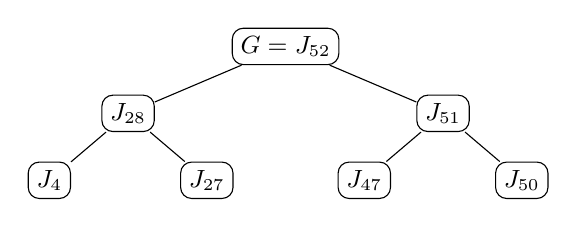
\begin{tikzpicture}[every node/.style={draw,rounded corners,inner sep=3pt,font=\small}]
\node (root) at (0,0) {$G=J_{52}$};
\node (left) at (-2,-.85) {$J_{28}$};
\node (right) at (2,-.85) {$J_{51}$};
\node (ll) at (-3,-1.70) {$J_4$};
\node (lr) at (-1,-1.70) {$J_{27}$};
\node (rl) at (1,-1.70) {$J_{47}$};
\node (rr) at (3,-1.70) {$J_{50}$};
\draw (root)--(left) (root)--(right) (left)--(ll) (left)--(lr)
      (right)--(rl) (right)--(rr);
\end{tikzpicture}
\caption{The upper part of the Ore composition tree. At each fork the
left graph supplies the deleted edge and the right graph the split vertex.
The complete table in Appendix~\ref{app:ore} specifies all 26 compositions.}
\label{fig:ore-tree}
\end{figure}

\begin{samepage}
The operation is the classical construction discussed by Kostochka and
Yancey~\cite[Section 1]{ky}; the following argument gives its
non-colorability property in the form used here.

\begin{lemma}\label{lem:ore}
If neither $A$ nor $B$ is three-colorable, their Ore composition is not
three-colorable.
\end{lemma}
\begin{proof}
Suppose the composite has a proper three-coloring $f$. Restrict $f$ to
$V(A)$. If $f(x)\ne f(y)$, restoring the deleted edge $xy$ gives a
proper three-coloring of $A$, a contradiction. Hence $f(x)=f(y)$.
Restrict $f$ to $V(B)\setminus\{z\}$ and give $z$ this common color.
Every neighbor of $z$ belonged to $N_x$ or $N_y$, and therefore has a
color different from that common color. Edges not incident with $z$
are unchanged. This is a proper three-coloring of $B$, again a
contradiction.
\end{proof}
\end{samepage}


The graph $K_4$ is not three-colorable: four pairwise adjacent vertices
need four distinct colors. Inducting over this explicit tree with
Lemma~\ref{lem:ore} proves that $G$ is not three-colorable. Starting with 27 copies of
$K_4$, each join reduces the sum of orders and the sum of sizes by one,
so the root has $27\cdot4-26=82$ vertices and
$27\cdot6-26=136$ edges.
Appendix~\ref{app:decomposition} verifies that the root is exactly $G$;
Appendices~\ref{app:graph} and~\ref{app:ore} give its edges, rotation
and complete construction tree.


\subsection{Planarity}\label{app:embedding}
The rotation system yields planarity by an orientable-surface argument.
Let $D=\{(u,v):uv\in E(G)\}$ be the darts. Write
$\rho_v(u)$ for the neighbor following $u$ in the cyclic order at $v$.
Let $F$ be the set of face-permutation orbits. The face permutation is
\[
   \phi(u,v)=(v,\rho_v(u)).
\]
The face permutation has 56 orbits. To justify this test,
place an oriented disk at every vertex, attach an untwisted band for
each edge according to the cyclic orders, and cap each boundary walk
with a disk. The result is a connected closed orientable surface with
a cellular embedding of $G$. The boundary walks are precisely the
orbits of $\phi$, so its Euler characteristic is
\[
   |V|-|E|+|F|=82-136+56=2.
\]
By the classification of closed orientable surfaces this surface is the
sphere. Deleting a point outside the embedded graph gives a plane
embedding. This proves planarity.


\subsection{Cycle exclusion}\label{sec:cycles}
Two independent complete enumerations of simple cycles give the counts in
Appendix~\ref{app:cycles}. Both find no cycle of length four or nine.
The first enumeration grows every simple path from its smallest vertex
$s$, using only other vertices greater than $s$. It records a closure
to $s$ when the path has at least three vertices and its second vertex
is smaller than its last. Every undirected simple cycle has a unique
smallest vertex and exactly two orientations, exactly one of which meets
this last test. Thus each cycle is counted once.
Appendix~\ref{app:cycles} gives the second enumeration and the counts.

\Needspace{22\baselineskip}
\subsection{Criticality and the edge bound}
The deletion colorings establish criticality, and the cited lower bound
then gives the stated edge minimum.
\begin{proof}[Proof of Theorem~\ref{thm:main}]
Induction from $K_4$ using Lemma~\ref{lem:ore} proves that $G$ is not
three-colorable and is a four-Ore graph. The rotation system has 56 faces,
so $82-136+56=2$; the orientable-surface argument in
Section~\ref{app:embedding} proves planarity. The enumerations in
Section~\ref{sec:cycles} and Appendix~\ref{app:cycles} find no simple four- or nine-cycle.
For an edge $e$, use the coloring of $G-e$ specified in
Appendix~\ref{app:decomposition}. The two endpoints of
$e$ necessarily have equal colors, since otherwise this would color
$G$. Recoloring one endpoint with a fourth color yields a proper
four-coloring of $G$. Together with the preceding induction, this proves
$\chi(G)=4$. The graph has no isolated vertices. Any proper subgraph
omits some edge of $G$, even if it omits a vertex, and is therefore a
subgraph of some $G-e$. Restricting that deletion coloring proves its
three-colorability. Consequently $G$ is four-critical.
Finally Kostochka and Yancey's bound gives
$|E(H)|\geq\lceil(5|V(H)|-2)/3\rceil$ for every four-critical graph $H$,
and $136=(5\cdot82-2)/3$ proves the edge minimum at order 82.
\end{proof}




\section{Computational verification}\label{sec:checks}
The computations used above establish the face orbits of the rotation,
the cycle counts in Appendix~\ref{app:cycles}, the compositions in
Appendix~\ref{app:ore}, and a proper three-coloring of $G-e$ for every edge
$e$. Appendix~\ref{app:additional} gives two further non-colorability arguments:
exact elimination of coloring constraints and a clausal proof of
unsatisfiability.

The formal graph $G$ has vertex set $\{0,\ldots,81\}$ and adjacency given
by exactly the 136 unordered edges in Appendix~\ref{app:graph}.
The Lean theorem \texttt{Steinberg.planar\_counterexample} states the
following conjunction for this graph:
\[
\begin{gathered}
G\text{ has a crossing-free straight-line drawing with rational coordinates};\\
\text{every simple cycle of }G\text{ has length different from four and nine};\\
\text{there is no proper coloring }V(G)\longrightarrow\{0,1,2\}.
\end{gathered}
\]
The formal planarity predicate, \texttt{RationalPlanar}, requires an
injective assignment of rational coordinate pairs to the vertices, with a
vertex on an edge segment only at an endpoint and edge segments meeting
only at a shared endpoint. Segments are closed real affine segments
between those rational points. The proof checks the existing drawing's
six-decimal coordinates as exact rationals. Mathlib's simple closed walks
and proper colorings supply the other two predicates; their conventions
agree with the introduction, including cycles with chords. This proves
the planar counterexample to the length-nine question directly from
these definitions.

The formal theorem has no hypotheses and is checked by Lean's kernel
using only its standard axioms. The exact axiom inventory, pinned versions
and build commands are in the accompanying
\href{https://raw.githubusercontent.com/6/clank-lab/main/results/steinberg-c4-c9/checks/README.md}{checking notes}.
Appendix~\ref{sec:replay} describes the formal non-colorability argument.
The remaining assertions of Theorem~\ref{thm:main}---Ore membership,
criticality and the edge minimum---use the written arguments in
Section~\ref{sec:ore}; the last uses Kostochka and Yancey's theorem.
The Ore construction, deletion colorings and other cycle counts also
have independent executable checks.

\clearpage\begin{appendices}
\section{The embedding certificate}\label{app:rotation}
Appendix~\ref{app:graph} gives the edge list and cyclic neighbor orders.
Tracing the face permutation of Section~\ref{app:embedding} gives 56 orbits,
after checking simplicity, the neighbor orders and connectedness.

\begin{figure}[H]
\centering
\begin{tikzpicture}[x=.0011875\linewidth,y=.0011875\linewidth]
\node[anchor=south west,inner sep=0] at (0,0)
  {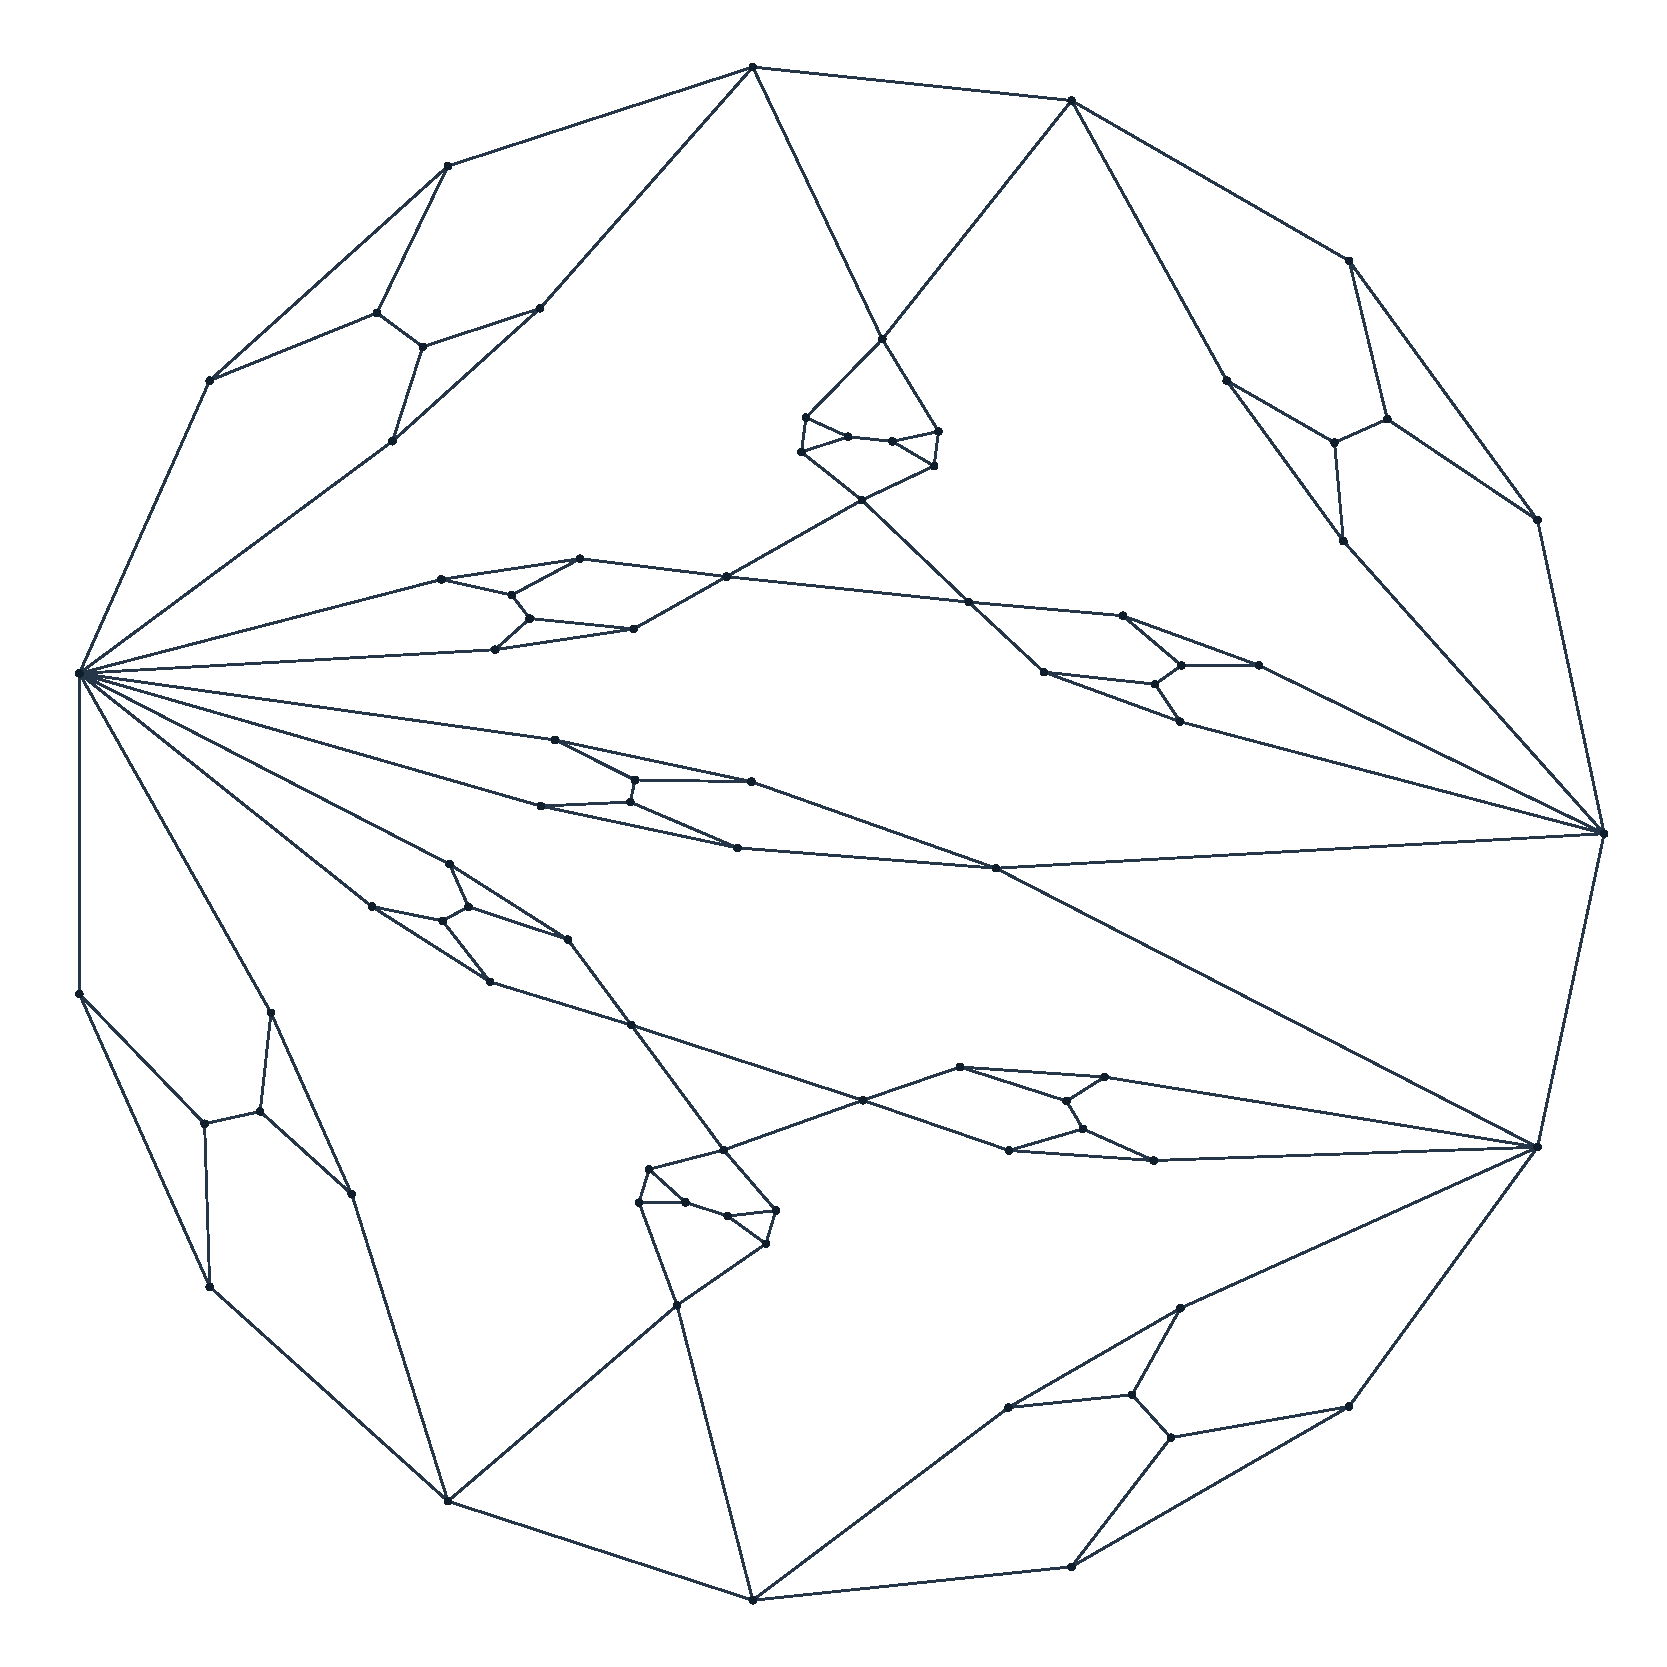
\includegraphics[width=0.95\linewidth]{../data/graph.pdf}};
\node[font=\fontsize{5}{5}\selectfont,fill=white,inner sep=.15pt] at (770.000000,400.000000) {0};
\node[font=\fontsize{5}{5}\selectfont,fill=white,inner sep=.15pt] at (738.011650,249.507310) {1};
\node[font=\fontsize{5}{5}\selectfont,fill=white,inner sep=.15pt] at (644.838345,540.380943) {2};
\node[font=\fontsize{5}{5}\selectfont,fill=white,inner sep=.15pt] at (738.011650,550.492690) {3};
\node[font=\fontsize{5}{5}\selectfont,fill=white,inner sep=.15pt] at (566.452283,453.751503) {4};
\node[font=\fontsize{5}{5}\selectfont,fill=white,inner sep=.15pt] at (604.282287,480.790146) {5};
\node[font=\fontsize{5}{5}\selectfont,fill=white,inner sep=.15pt] at (478.054355,383.409020) {6};
\node[font=\fontsize{5}{5}\selectfont,fill=white,inner sep=.15pt] at (38.085240,476.927440) {7};
\node[font=\fontsize{5}{5}\selectfont,fill=white,inner sep=.15pt] at (237.660169,488.308987) {8};
\node[font=\fontsize{5}{5}\selectfont,fill=white,inner sep=.15pt] at (211.832965,522.038270) {9};
\node[font=\fontsize{5}{5}\selectfont,fill=white,inner sep=.15pt] at (100.663710,617.480450) {10};
\node[font=\fontsize{5}{5}\selectfont,fill=white,inner sep=.15pt] at (188.386138,588.355972) {11};
\node[font=\fontsize{5}{5}\selectfont,fill=white,inner sep=.15pt] at (266.422789,444.983980) {12};
\node[font=\fontsize{5}{5}\selectfont,fill=white,inner sep=.15pt] at (259.674517,413.235905) {13};
\node[font=\fontsize{5}{5}\selectfont,fill=white,inner sep=.15pt] at (38.085240,323.072560) {14};
\node[font=\fontsize{5}{5}\selectfont,fill=white,inner sep=.15pt] at (130.069798,313.999464) {15};
\node[font=\fontsize{5}{5}\selectfont,fill=white,inner sep=.15pt] at (215.776680,385.355380) {16};
\node[font=\fontsize{5}{5}\selectfont,fill=white,inner sep=.15pt] at (178.463421,365.047041) {17};
\node[font=\fontsize{5}{5}\selectfont,fill=white,inner sep=.15pt] at (553.760767,243.105403) {18};
\node[font=\fontsize{5}{5}\selectfont,fill=white,inner sep=.15pt] at (530.198937,283.193281) {19};
\node[font=\fontsize{5}{5}\selectfont,fill=white,inner sep=.15pt] at (647.578470,125.036350) {20};
\node[font=\fontsize{5}{5}\selectfont,fill=white,inner sep=.15pt] at (566.572892,172.170875) {21};
\node[font=\fontsize{5}{5}\selectfont,fill=white,inner sep=.15pt] at (514.336290,751.891090) {22};
\node[font=\fontsize{5}{5}\selectfont,fill=white,inner sep=.15pt] at (588.824019,617.478098) {23};
\node[font=\fontsize{5}{5}\selectfont,fill=white,inner sep=.15pt] at (647.578470,674.963650) {24};
\node[font=\fontsize{5}{5}\selectfont,fill=white,inner sep=.15pt] at (423.527585,637.330284) {25};
\node[font=\fontsize{5}{5}\selectfont,fill=white,inner sep=.15pt] at (361.324640,767.973140) {26};
\node[font=\fontsize{5}{5}\selectfont,fill=white,inner sep=.15pt] at (464.989263,511.156791) {27};
\node[font=\fontsize{5}{5}\selectfont,fill=white,inner sep=.15pt] at (501.092840,477.570816) {28};
\node[font=\fontsize{5}{5}\selectfont,fill=white,inner sep=.15pt] at (538.922844,504.609458) {29};
\node[font=\fontsize{5}{5}\selectfont,fill=white,inner sep=.15pt] at (348.759221,523.373067) {30};
\node[font=\fontsize{5}{5}\selectfont,fill=white,inner sep=.15pt] at (413.677878,560.117998) {31};
\node[font=\fontsize{5}{5}\selectfont,fill=white,inner sep=.15pt] at (640.571853,587.710324) {32};
\node[font=\fontsize{5}{5}\selectfont,fill=white,inner sep=.15pt] at (665.893145,598.976541) {33};
\node[font=\fontsize{5}{5}\selectfont,fill=white,inner sep=.15pt] at (554.483446,471.723780) {34};
\node[font=\fontsize{5}{5}\selectfont,fill=white,inner sep=.15pt] at (567.093448,480.736660) {35};
\node[font=\fontsize{5}{5}\selectfont,fill=white,inner sep=.15pt] at (304.233165,498.261622) {36};
\node[font=\fontsize{5}{5}\selectfont,fill=white,inner sep=.15pt] at (278.405961,531.990904) {37};
\node[font=\fontsize{5}{5}\selectfont,fill=white,inner sep=.15pt] at (450.486762,593.018397) {38};
\node[font=\fontsize{5}{5}\selectfont,fill=white,inner sep=.15pt] at (386.829553,599.709038) {39};
\node[font=\fontsize{5}{5}\selectfont,fill=white,inner sep=.15pt] at (254.261245,503.278437) {40};
\node[font=\fontsize{5}{5}\selectfont,fill=white,inner sep=.15pt] at (245.652177,514.521531) {41};
\node[font=\fontsize{5}{5}\selectfont,fill=white,inner sep=.15pt] at (215.000000,720.429250) {42};
\node[font=\fontsize{5}{5}\selectfont,fill=white,inner sep=.15pt] at (259.205886,652.122282) {43};
\node[font=\fontsize{5}{5}\selectfont,fill=white,inner sep=.15pt] at (180.931283,649.947938) {44};
\node[font=\fontsize{5}{5}\selectfont,fill=white,inner sep=.15pt] at (202.919336,633.709364) {45};
\node[font=\fontsize{5}{5}\selectfont,fill=white,inner sep=.15pt] at (448.376111,576.472907) {46};
\node[font=\fontsize{5}{5}\selectfont,fill=white,inner sep=.15pt] at (384.718902,583.163548) {47};
\node[font=\fontsize{5}{5}\selectfont,fill=white,inner sep=.15pt] at (428.337354,588.305012) {48};
\node[font=\fontsize{5}{5}\selectfont,fill=white,inner sep=.15pt] at (407.118285,590.535225) {49};
\node[font=\fontsize{5}{5}\selectfont,fill=white,inner sep=.15pt] at (414.159073,272.019732) {50};
\node[font=\fontsize{5}{5}\selectfont,fill=white,inner sep=.15pt] at (484.363787,247.929493) {51};
\node[font=\fontsize{5}{5}\selectfont,fill=white,inner sep=.15pt] at (460.801956,288.017371) {52};
\node[font=\fontsize{5}{5}\selectfont,fill=white,inner sep=.15pt] at (347.369490,248.161706) {53};
\node[font=\fontsize{5}{5}\selectfont,fill=white,inner sep=.15pt] at (303.008850,308.134671) {54};
\node[font=\fontsize{5}{5}\selectfont,fill=white,inner sep=.15pt] at (361.324640,32.026860) {55};
\node[font=\fontsize{5}{5}\selectfont,fill=white,inner sep=.15pt] at (514.336290,48.108910) {56};
\node[font=\fontsize{5}{5}\selectfont,fill=white,inner sep=.15pt] at (484.043091,124.522250) {57};
\node[font=\fontsize{5}{5}\selectfont,fill=white,inner sep=.15pt] at (215.000000,79.570750) {58};
\node[font=\fontsize{5}{5}\selectfont,fill=white,inner sep=.15pt] at (324.962604,173.618580) {59};
\node[font=\fontsize{5}{5}\selectfont,fill=white,inner sep=.15pt] at (360.701885,424.944319) {60};
\node[font=\fontsize{5}{5}\selectfont,fill=white,inner sep=.15pt] at (353.953613,393.196244) {61};
\node[font=\fontsize{5}{5}\selectfont,fill=white,inner sep=.15pt] at (304.798112,425.766223) {62};
\node[font=\fontsize{5}{5}\selectfont,fill=white,inner sep=.15pt] at (302.548688,415.183531) {63};
\node[font=\fontsize{5}{5}\selectfont,fill=white,inner sep=.15pt] at (519.808833,258.280341) {64};
\node[font=\fontsize{5}{5}\selectfont,fill=white,inner sep=.15pt] at (511.954890,271.642967) {65};
\node[font=\fontsize{5}{5}\selectfont,fill=white,inner sep=.15pt] at (561.974516,110.077377) {66};
\node[font=\fontsize{5}{5}\selectfont,fill=white,inner sep=.15pt] at (543.424720,130.668688) {67};
\node[font=\fontsize{5}{5}\selectfont,fill=white,inner sep=.15pt] at (100.663710,182.519550) {68};
\node[font=\fontsize{5}{5}\selectfont,fill=white,inner sep=.15pt] at (168.830731,226.941079) {69};
\node[font=\fontsize{5}{5}\selectfont,fill=white,inner sep=.15pt] at (372.415771,219.107707) {70};
\node[font=\fontsize{5}{5}\selectfont,fill=white,inner sep=.15pt] at (311.540681,238.887247) {71};
\node[font=\fontsize{5}{5}\selectfont,fill=white,inner sep=.15pt] at (98.207686,260.764452) {72};
\node[font=\fontsize{5}{5}\selectfont,fill=white,inner sep=.15pt] at (124.899616,266.655857) {73};
\node[font=\fontsize{5}{5}\selectfont,fill=white,inner sep=.15pt] at (272.546025,349.185501) {74};
\node[font=\fontsize{5}{5}\selectfont,fill=white,inner sep=.15pt] at (235.232766,328.877162) {75};
\node[font=\fontsize{5}{5}\selectfont,fill=white,inner sep=.15pt] at (224.853890,364.927842) {76};
\node[font=\fontsize{5}{5}\selectfont,fill=white,inner sep=.15pt] at (212.416137,358.158396) {77};
\node[font=\fontsize{5}{5}\selectfont,fill=white,inner sep=.15pt] at (367.614295,203.134180) {78};
\node[font=\fontsize{5}{5}\selectfont,fill=white,inner sep=.15pt] at (306.739206,222.913720) {79};
\node[font=\fontsize{5}{5}\selectfont,fill=white,inner sep=.15pt] at (349.296906,216.449052) {80};
\node[font=\fontsize{5}{5}\selectfont,fill=white,inner sep=.15pt] at (329.005210,223.042232) {81};
\end{tikzpicture}
\caption{The counterexample, with vertex numbers from the accompanying
\href{https://raw.githubusercontent.com/6/clank-lab/main/results/steinberg-c4-c9/data/graph.svg}{SVG drawing}.
The drawing was generated from, and checked against, the edge and rotation
data in Appendix~\ref{app:graph}; its rational coordinates are also checked in Lean.}
\label{fig:graph}
\end{figure}

\paragraph{Drawing.} The figure is obtained by applying Tutte's barycentric
method to a triangulation of the bounded faces, using temporary centers,
and then omitting the added vertices and edges. For background see Tutte's
``How to Draw a Graph''~\cite{tutte}. The finite-decimal coordinates are exact
rationals, checked in Lean as described in Section~\ref{sec:checks}.

\section{Excluding cycles}\label{app:cycles}
An independent enumeration checks the cycle counts used in
Section~\ref{sec:cycles}, counting undirected simple cycles without multiplicity.
The second enumeration instead chooses an edge $(s,t)$ with $s<t$, and
enumerates simple $s$--$t$ paths avoiding that edge, with all other vertices
greater than $s$. Closing by $ts$ gives a simple cycle. A cycle whose
smallest vertex is $s$ is found twice, once for each of its two edges at
$s$; division by two gives the count. Each raw count is even. Both enumerations run through length 14 and
return the same table:
\begin{center}\small
\begin{tabular}{c|rrrrrrrrrrrr}
length&3&4&5&6&7&8&9&10&11&12&13&14\\\hline
count&27&0&22&55&44&11&0&0&64&320&832&1824
\end{tabular}
\end{center}
In particular there is no $C_4$, $C_9$ or $C_{10}$.

\section{The construction and deletion colorings}\label{app:decomposition}
The construction table identifies the graph used in the Ore induction,
and the deletion colorings certify its criticality.
The tree printed in Appendix~\ref{app:ore} has 27 leaves and 26 internal
nodes. Each leaf gives four distinct vertices and all six edges of a
$K_4$. Every internal node gives two earlier, disjoint operands, an edge
$xy$ of the first, a vertex $z$ of the second, and two nonempty sets
$N_x,N_y$ partitioning $N_B(z)$. Applying the operation in
Section~\ref{sec:ore} at each node gives the root graph. Every non-root
node occurs as an operand exactly once. At the root the vertex labels
are $0,\ldots,81$ and the edges are exactly those in Appendix~\ref{app:graph},
with the identity correspondence on vertices.

For each of the 136 edges $e$, the
\href{https://raw.githubusercontent.com/6/clank-lab/main/results/steinberg-c4-c9/data/deletion-colorings.json}{accompanying deletion-coloring data}
gives a vector
$(c_0,\ldots,c_{81})\in\{0,1,2\}^{82}$ whose coordinates differ across
every edge other than $e$. These are the deletion colorings used in the
proof of Theorem~\ref{thm:main}; the checking notes specify their location
and verification.
\subsection{Edge count and other cycle lengths}
The tree proves that $G$ is a four-Ore graph.
The bound used in the main proof is Kostochka and Yancey's
Theorem 3~\cite{kybound}, also stated as Theorem 4 in~\cite{ky}. Every four-critical graph $H$ satisfies
\[
 |E(H)|\geq\left\lceil\frac{5|V(H)|-2}{3}\right\rceil.
\]
For the graph in this paper,
\[
 136=\frac{5\cdot82-2}{3}.
\]
The general four-Ore construction and its edge count are discussed in
Kostochka and Yancey's Section 1~\cite{ky}. Thus the edge minimum in
Theorem~\ref{thm:main} is at fixed order 82, among all four-critical graphs.
The cycle table also gives the exclusion of $C_{10}$ and the presence of
$C_5,C_6,C_7,C_8$.

\clearpage
\section{Two additional checks of non-colorability}\label{app:additional}
These checks establish non-colorability independently of the Ore induction.

\subsection{Exact constraint elimination}
A relation's \emph{scope} is the set of vertices whose colors it specifies.
The \emph{interaction graph} joins two remaining vertices when they occur
in the scope of a common relation.

For each edge $uv$ start with the relation
$R_{uv}=\{(a,b)\in\{0,1,2\}^2:a\ne b\}$.
Maintain a conjunction of relations on the remaining vertices. To
eliminate $v$, collect all relations mentioning it, let $S$ be the union
of their scopes minus $v$, and replace them by the relation
\[
 R_S=\{a\in\{0,1,2\}^S:
          \exists c\in\{0,1,2\}\;
          \bigwedge_{R\text{ mentioning }v}R(a,v=c)\}.
\]
All other relations remain. The new conjunction is exactly the
existential projection of the old one. Induction on eliminations shows
that satisfiability is preserved. An empty relation proves that no
coloring exists; a nonempty relation on the empty scope is a tautology
and may be discarded.

Each elimination enumerates all $3^{|S|}$ assignments and all three
values of $c$. A vertex of minimum degree in the current interaction
graph is chosen, breaking ties by vertex label. This choice affects cost,
not correctness. For this graph an empty relation is reached; the largest
remaining scope $S$ has size three.

\subsection{Exact graph-to-CNF reduction and symmetry}
The coloring constraints form a conjunction of clauses, or conjunctive
normal form (CNF).
Independently introduce Boolean variables $x_{v,c}$, numbered $3v+c+1$,
for $0\leq v<82$ and $c\in\{0,1,2\}$. The generator adds the clauses
\begin{align*}
 &x_{v,0}\lor x_{v,1}\lor x_{v,2}&&\text{for each }v,\\
 &\neg x_{v,a}\lor\neg x_{v,b}&&\text{for each }v\text{ and }0\leq a<b<3,\\
 &\neg x_{u,c}\lor\neg x_{v,c}&&\text{for each }uv\in E(G)\text{ and }c.
\end{align*}
The first two lines specify exactly one color at each vertex, and the
third specifies distinct colors across every edge. Assigning the unique
true color is therefore a bijection between satisfying assignments of
these clauses and proper three-colorings of $G$.

The lexicographically first triangle is $(0,1,6)$. The generator also
adds $x_{0,0}$, $x_{1,1}$ and $x_{6,2}$, that is, unit clauses $1$, $5$
and $21$. Every proper coloring gives distinct colors to this triangle.
There is a permutation of the three color names taking them, in this
order, to $0,1,2$; the other clauses are invariant under this permutation.
Adding these units thus preserves satisfiability.

The resulting formula has a clausal proof ending with the empty clause,
generated with CaDiCaL~\cite{cadical} and checked by DRAT-trim~\cite{drat}.
Each clause addition satisfies a checked redundancy condition preserving
satisfiability; a clause deletion weakens the formula. The final empty
clause therefore proves unsatisfiability. Together with the color-permutation
argument and the exact reduction above, this proves that $G$ has no proper
three-coloring. The formula and proof, their sizes and the checking commands
are given in the checking notes.

\section{Formal verification}\label{sec:replay}
The formal proof certifies non-three-colorability by deducing a
contradiction from the coloring clauses. Its coloring formula has the
edge and vertex clauses of Appendix~\ref{app:additional}, without units
that prescribe a color for an individual vertex. The formal
reduction proves that a proper coloring would satisfy this formula.
Equality of the formula produced by the reduction with the certificate's
input is proved in Lean.

Unit propagation assigns the only remaining literal of a clause when
all its other literals are false. Clause additions are justified by
reverse unit propagation: assuming
the negation of a proposed clause, unit propagation in previously justified
clauses yields a contradiction. The formal proof establishes this
implication and applies it to every addition. Hints specify the clauses
used in these deductions. Deletion instructions leave earlier clauses
available; every such clause remains entailed by the original input.
The final empty clause proves unsatisfiability of that input.

The use of hints follows Cruz-Filipe, Heule, Hunt, Kaufmann and
Schneider-Kamp~\cite[abstract]{lrat}, whose format extends DRAT, a
clausal proof format allowing clause additions and deletions,
``with hints that facilitate a simple and fast validation algorithm.''
The checking notes give the exact certificate formats and formal theorem
names.

\clearpage
\section{Explicit graph and rotation}\label{app:graph}
The graph list gives every edge, and the rotation gives every neighbor
in cyclic order. Together they specify the labeled graph and its embedding.
\subsection*{Graph}
\begin{multicols}{3}\footnotesize
\VerbatimInput[firstline=2]{../data/graph.txt}
\end{multicols}
\clearpage
\subsection*{Rotation}
\begin{multicols}{2}\footnotesize
\VerbatimInput[firstline=2]{../data/rotation.txt}
\end{multicols}
\clearpage
\section{The explicit Ore tree}\label{app:ore}
Each leaf row specifies the four vertices of a complete graph. Each
internal row specifies the two operand indices, then $x,y,z,N_x,N_y$
in the notation of Section~\ref{sec:ore}. Operands are disjoint at every
composition. The root graph is $G$, with the identity correspondence on
$0,\ldots,81$.
\begin{center}\small
\begin{tabular}{r|l}
node & vertices of $K_4$\\\hline
0 & $0,1,6,7$\\
1 & $12,60,62,84$\\
2 & $13,61,63,85$\\
5 & $50,53,54,83$\\
6 & $16,74,76,89$\\
7 & $17,75,77,90$\\
10 & $55,58,59,88$\\
11 & $14,68,72,92$\\
12 & $15,69,73,93$\\
15 & $20,56,66,91$\\
16 & $21,57,67,94$\\
20 & $70,78,80,87$\\
21 & $71,79,81,95$\\
24 & $18,51,64,86$\\
25 & $19,52,65,96$\\
29 & $22,25,26,82$\\
30 & $10,42,44,100$\\
31 & $11,43,45,101$\\
34 & $27,30,31,99$\\
35 & $8,36,40,103$\\
36 & $9,37,41,104$\\
39 & $4,28,34,102$\\
40 & $5,29,35,105$\\
44 & $38,46,48,98$\\
45 & $39,47,49,106$\\
48 & $2,23,32,97$\\
49 & $3,24,33,107$\\
\end{tabular}
\end{center}
\begin{center}\scriptsize
\begin{tabular}{r|rr|rr|r|l|l}
node & $A$ & $B$ & $x$ & $y$ & $z$ & $N_x$ & $N_y$\\\hline
3 & 1 & 2 & 62 & 84 & 85 & $63$ & $13,61$\\
4 & 0 & 3 & 6 & 7 & 84 & $60,61$ & $12,13$\\
8 & 6 & 7 & 76 & 89 & 90 & $77$ & $17,75$\\
9 & 5 & 8 & 54 & 83 & 89 & $74,75$ & $16,17$\\
13 & 11 & 12 & 72 & 92 & 93 & $73$ & $15,69$\\
14 & 10 & 13 & 58 & 88 & 92 & $68,69$ & $14,15$\\
17 & 15 & 16 & 66 & 91 & 94 & $67$ & $21,57$\\
18 & 14 & 17 & 55 & 88 & 91 & $56,57$ & $20,21$\\
19 & 9 & 18 & 53 & 83 & 88 & $59$ & $14,15,20,21$\\
22 & 20 & 21 & 80 & 87 & 95 & $81$ & $71,79$\\
23 & 19 & 22 & 53 & 59 & 87 & $70,71$ & $78,79$\\
26 & 24 & 25 & 64 & 86 & 96 & $65$ & $19,52$\\
27 & 23 & 26 & 50 & 83 & 86 & $51,52$ & $18,19$\\
28 & 4 & 27 & 1 & 7 & 83 & $18,19,20,21$ & $14,15,16,17$\\
32 & 30 & 31 & 44 & 100 & 101 & $45$ & $11,43$\\
33 & 29 & 32 & 26 & 82 & 100 & $42,43$ & $10,11$\\
37 & 35 & 36 & 40 & 103 & 104 & $41$ & $9,37$\\
38 & 34 & 37 & 30 & 99 & 103 & $36,37$ & $8,9$\\
41 & 39 & 40 & 34 & 102 & 105 & $35$ & $5,29$\\
42 & 38 & 41 & 27 & 99 & 102 & $28,29$ & $4,5$\\
43 & 33 & 42 & 25 & 82 & 99 & $31$ & $4,5,8,9$\\
46 & 44 & 45 & 48 & 98 & 106 & $49$ & $39,47$\\
47 & 43 & 46 & 25 & 31 & 98 & $38,39$ & $46,47$\\
50 & 48 & 49 & 32 & 97 & 107 & $33$ & $3,24$\\
51 & 47 & 50 & 22 & 82 & 97 & $23,24$ & $2,3$\\
52 & 28 & 51 & 0 & 7 & 82 & $2,3,4,5$ & $8,9,10,11$\\
\end{tabular}
\end{center}

\end{appendices}

\section*{Acknowledgments}
Kostochka and Yancey describe the construction as ``found in Dirac's
paper'' and ``used by Gallai \ldots{} and Haj\'os'', and say that Ore
``used it for a composition of complete graphs''~\cite[Section 1]{ky}. The sharp edge bound is
Kostochka and Yancey's~\cite[Theorem 3]{kybound}, also reproduced as
Theorem 4 in~\cite{ky}.
We acknowledge the researchers cited above for posing and developing
the forbidden-cycle questions, and Cohen-Addad and coauthors for their
disproof of Steinberg's conjecture. The formalization uses
\href{https://github.com/leanprover/lean4}{Lean 4 and its standard library}
and \href{https://github.com/leanprover-community/mathlib4}{Mathlib},
developed by their contributors. The SAT certificate was generated with CaDiCaL~\cite{cadical}
and checked with Heule and Wetzler's DRAT-trim~\cite{drat}.
\clearpage
\begin{thebibliography}{99}
\bibitem{lu} H. Lu, Y. Wang, W. Wang, Y. Bu, M. Montassier and A. Raspaud.
On the 3-colorability of planar graphs without 4-, 7- and 9-cycles.
\emph{Discrete Math.} 309 (2009), 4596--4607.
\href{https://doi.org/10.1016/j.disc.2009.02.030}{doi:10.1016/j.disc.2009.02.030}.
\bibitem{kjw} Y. Kang, L. Jin and Y. Wang.
The 3-colorability of planar graphs without cycles of length 4, 6 and 9.
\emph{Discrete Math.} 339 (2016), 299--307.
\href{https://arxiv.org/abs/1506.04629v1}{arXiv:1506.04629} version 1 (2015), Problem 1.2 and Theorem 1.4.
\bibitem{jklw} Y. Kang, L. Jin, P. Liu and Y. Wang.
$(1,0,0)$-colorability of planar graphs without cycles of length 4 or 6.
\emph{Discrete Math.} 345 (2022), 112758.
\href{https://doi.org/10.1016/j.disc.2021.112758}{doi:10.1016/j.disc.2021.112758};
\href{https://arxiv.org/abs/2001.00166v1}{arXiv:2001.00166v1} (2020), Problem 1.2, with author order L. Jin, Y. Kang, P. Liu and Y. Wang.
\bibitem{steinberg} V. Cohen-Addad, M. Hebdige, D. Král', Z. Li and E. Salgado.
Steinberg's conjecture is false.
\emph{J. Combin. Theory Ser. B} 122 (2017), 452--456.
\href{https://arxiv.org/abs/1604.05108v2}{arXiv:1604.05108} version 2 (2016), Theorem 3 and Figure 1.
\bibitem{kjz} Y. Kang, L. Jin and X. Zhu.
Planar graphs having no cycle of length 4, 7, or 9 are DP-3-colorable.
\emph{J. Graph Theory} 107 (2024), 344--358.
\href{https://doi.org/10.1002/jgt.23123}{doi:10.1002/jgt.23123};
\href{https://arxiv.org/abs/2303.04657v1}{arXiv:2303.04657} version 1 (2023),
entitled ``DP-3-colorability of planar graphs without cycles of length 4, 7 or 9'',
Theorem 1.1 and Corollary 1.2.
\bibitem{dai} L. Dai, Y. Wang and J. Xu.
Every planar graph without cycles of length 4 or 9 is $(1,1,0)$-colorable.
\emph{Discrete Math.} 340 (2017), 2108--2122.
\href{https://doi.org/10.1016/j.disc.2017.04.006}{doi:10.1016/j.disc.2017.04.006}.
\bibitem{nie} M. Chen, L. Dai, J. Nie, Y. Wang and W. Yu.
Planar graphs without cycles of length 4 or 9 are $(2,0,0)$-colorable.
\emph{Sci. Sin. Math.} 50 (2020), 317--338, Theorem 1.4.
\href{https://doi.org/10.1360/N012018-00129}{doi:10.1360/N012018-00129}.
\bibitem{xiao} Y. Xiao and M. Huang.
A weak DP-coloring of planar graphs without 4- and 9-cycles.
\emph{Discrete Appl. Math.} 342 (2024), 391--397.
\href{https://doi.org/10.1016/j.dam.2023.10.004}{doi:10.1016/j.dam.2023.10.004}.
\bibitem{ang} R. K. Ang and Z. H. Leo.
Exploring the Weak Steinberg's Conjecture.
In \emph{Proceedings of the 11th IRC Conference on Science, Engineering
and Technology} (IRC-SET 2025), Proceedings in Technology Transfer,
Springer, Singapore (2026), 435--443.
\href{https://doi.org/10.1007/978-981-95-9630-0_37}{doi:10.1007/978-981-95-9630-0\_37}.
\bibitem{survey} Y. Bu, W. Wang and Y. Wang.
On Coloring Problems. In \emph{Handbook of Combinatorial Optimization},
1--138. Online December 17, 2024; print 2025.
\href{https://doi.org/10.1007/978-1-4614-6624-6_59-1}{doi:10.1007/978-1-4614-6624-6\_59-1}.
\bibitem{bordeaux} X. Li, L. Niu and F. Tian.
On the strong Bordeaux Conjecture.
\emph{Discrete Math.} 349 (2026), 114818.
\href{https://doi.org/10.1016/j.disc.2025.114818}{doi:10.1016/j.disc.2025.114818}.
\bibitem{kybound} A. Kostochka and M. Yancey.
Ore's Conjecture on color-critical graphs is almost true.
\emph{J. Combin. Theory Ser. B} 109 (2014), 73--101.
\href{https://arxiv.org/abs/1209.1050v1}{arXiv:1209.1050v1} (2012), Theorem 3;
\href{https://doi.org/10.1016/j.jctb.2014.05.002}{doi:10.1016/j.jctb.2014.05.002}.
\bibitem{ky} A. Kostochka and M. Yancey.
A Brooks-type result for sparse critical graphs.
\emph{Combinatorica} 38 (2018), 887--934.
\href{https://arxiv.org/abs/1408.0846v3}{arXiv:1408.0846}, version 3 (2017),
Theorem 4 and DHGO-composition and four-Ore graphs.
\bibitem{drat} N. Wetzler, M. J. H. Heule and W. A. Hunt, Jr.
DRAT-trim: Efficient checking and trimming using expressive clausal proofs.
\emph{SAT 2014}, LNCS 8561, 422--429.
\href{https://doi.org/10.1007/978-3-319-09284-3_31}{doi:10.1007/978-3-319-09284-3\_31}.
\bibitem{cadical} A. Biere, K. Fazekas, M. Fleury and M. Heisinger.
CaDiCaL, Kissat, Paracooba, Plingeling and Treengeling entering the
SAT Competition 2020. \emph{Proc. SAT Competition 2020}, 50--53.
\href{https://fmv.jku.at/papers/BiereFazekasFleuryHeisinger-SAT-Competition-2020-solvers.pdf}{Authors' chapter}.
\href{https://github.com/arminbiere/cadical}{CaDiCaL source and contributors}.
\bibitem{lrat} L. Cruz-Filipe, M. J. H. Heule, W. A. Hunt, Jr.,
M. Kaufmann and P. Schneider-Kamp.
Efficient Certified RAT Verification.
\emph{CADE 2017}, LNCS 10395, 220--236.
\href{https://doi.org/10.1007/978-3-319-63046-5_14}{doi:10.1007/978-3-319-63046-5\_14};
\href{https://www.cs.cmu.edu/~mheule/publications/lrat.pdf}{author-hosted CADE 2017 version}.
\bibitem{tutte} W. T. Tutte. How to Draw a Graph.
\emph{Proc. London Math. Soc.} (3) 13 (1963), 743--767.
\href{https://doi.org/10.1112/plms/s3-13.1.743}{doi:10.1112/plms/s3-13.1.743}.
\end{thebibliography}

\end{document}
